% Based on KACTL (Anders Sjoqvist, Ulf Lundstrom), CC0, plus beginner basics
% and number theory theory.

\chapter{Mathematics}

\section{Basics (read first)}
\textbf{Limits:} \texttt{int} $\le 2^{31}-1 \approx 2.1\cdot10^9$,
\texttt{ll} $\approx 9.2\cdot10^{18}$, \texttt{ull} $\approx 1.8\cdot10^{19}$,
\texttt{\_\_int128} $\approx 1.7\cdot10^{38}$. \texttt{double} is exact for integers up to
$2^{53}\approx 9\cdot10^{15}$ (15--16 digits), \texttt{long double} up to $2^{64}$ (18--19 digits).
$2^{10}\approx10^3$, $2^{20}\approx10^6$, $2^{30}\approx10^9$, $2^{60}\approx10^{18}$;
$\log_2 10^{18}\approx 60$. $10^5\cdot10^5$ overflows \texttt{int}: write \texttt{1LL * a * b}.

\textbf{Modular rules:} $(a\pm b) \bmod m$ and $ab \bmod m$ can be reduced at every step.
Subtraction: \texttt{((a - b) \% m + m) \% m} (C++ \texttt{\%} keeps the sign).
Division is NOT allowed directly: $a/b \equiv a\cdot b^{-1}$, and $b^{-1}$ exists iff
$\gcd(b,m)=1$; for prime $p$, $b^{-1} = b^{p-2}$. For $m > 3\cdot10^9$ multiply with
\texttt{\_\_int128}. Exponents reduce mod $p-1$ (if $p \nmid a$), not mod $p$.

\textbf{Floor / ceil:} for $a\ge0, b>0$: $\lceil a/b\rceil = \lfloor (a+b-1)/b\rfloor$.
$\lfloor\lfloor n/a\rfloor/b\rfloor = \lfloor n/(ab)\rfloor$.
Multiples of $k$ in $[l, r]$ ($l \ge 1$): $\lfloor r/k\rfloor - \lfloor (l-1)/k\rfloor$.
$x \bmod k = x - k\lfloor x/k\rfloor$. Negative numbers: use floorDiv / ceilDiv (Misc.h).

\textbf{Bits:} \texttt{x \& (x-1)} clears the lowest set bit, \texttt{x \& -x} keeps it;
$x$ is a power of 2 iff \texttt{x \&\& !(x \& (x-1))}.
$a+b = (a \oplus b) + 2(a \,\&\, b) = (a \,|\, b) + (a \,\&\, b)$. $a\oplus a=0$.
$1\oplus2\oplus\dots\oplus n = n, 1, n+1, 0$ for $n \bmod 4 = 0,1,2,3$.
Submasks of $m$: \texttt{for (s = m; s; s = (s - 1) \& m)}.

\textbf{Progressions:} arithmetic $a_1..a_n$: sum $= n(a_1+a_n)/2$, $a_n = a_1 + (n-1)d$.
Geometric: $a + ar + \dots + ar^{n-1} = a\frac{r^n-1}{r-1}$ (mod $p$: multiply by $(r-1)^{-1}$,
or use matrix power / divide and conquer if $r \equiv 1$).

\section{Equations}
\[ax^2+bx+c=0 \Rightarrow x = \frac{-b\pm\sqrt{b^2-4ac}}{2a}\]
The extremum is given by $x = -b/2a$.
\[\begin{aligned}ax+by=e\\cx+dy=f\end{aligned}
\Rightarrow
\begin{aligned}x=\dfrac{ed-bf}{ad-bc}\\y=\dfrac{af-ec}{ad-bc}\end{aligned}\]
In general, given an equation $Ax = b$, the solution to a variable $x_i$ is given by
\[x_i = \frac{\det A_i'}{\det A} \]
where $A_i'$ is $A$ with the $i$'th column replaced by $b$.

\section{Recurrences}
If $a_n = c_1 a_{n-1} + \dots + c_k a_{n-k}$, and $r_1, \dots, r_k$ are distinct roots of
$x^k - c_1 x^{k-1} - \dots - c_k$, there are $d_1, \dots, d_k$ s.t.
\[a_n = d_1r_1^n + \dots + d_kr_k^n. \]
Non-distinct roots $r$ become polynomial factors, e.g. $a_n = (d_1n + d_2)r^n$.
Compute $a_n$ fast with a $k\times k$ matrix power (Matrix.h).

\section{Number theory}
\subsection{Divisibility and gcd}
$\gcd(a,b)=\gcd(b, a \bmod b)$, $\gcd(a,b)\cdot\text{lcm}(a,b)=ab$
(compute $\text{lcm}$ as $a/\gcd\cdot b$). $\gcd(a,b)=\gcd(a, b-a)$.
$\gcd(a^m-1, a^n-1) = a^{\gcd(m,n)}-1$. $\gcd(F_m,F_n)=F_{\gcd(m,n)}$.
Over many numbers, prefix gcds change at most $\log(\max)$ times.

\textbf{Bezout / linear Diophantine:} $ax+by=c$ has integer solutions iff $g=\gcd(a,b)\mid c$.
From extgcd (the \emph{Pulverizer}: \texttt{euclid} / \texttt{diophantine} in Euclid.h)
$ax_0+by_0=g$: $x = x_0\frac cg + k\frac bg$, $y = y_0\frac cg - k\frac ag$, $k\in\mathbb Z$.
By hand, run Euclid and keep each remainder as a combination of $a$ and $b$:
$r_i = r_{i-2} - q_i r_{i-1}$, so $(x_i, y_i) = (x_{i-2} - q_ix_{i-1},\ y_{i-2} - q_iy_{i-1})$,
starting from $(1,0)$ for $a$ and $(0,1)$ for $b$.

\textbf{CRT:} $x\equiv a_i \pmod{m_i}$ is solvable iff $a_i\equiv a_j \pmod{\gcd(m_i,m_j)}$ for all
$i,j$; the solution is unique mod $\text{lcm}(m_i)$. Merge two at a time (CRT.h).

\subsection{Theorems}
\textbf{Fermat:} $p$ prime, $p\nmid a$: $a^{p-1}\equiv1 \pmod p$.
\textbf{Euler:} $\gcd(a,n)=1 \Rightarrow a^{\phi(n)}\equiv 1 \pmod n$.
\textbf{Power towers:} $a^{e} \equiv a^{(e \bmod \phi(n)) + \phi(n)} \pmod n$ for $e \ge \log_2 n$
(any $a$). \textbf{Wilson:} $(p-1)!\equiv -1 \pmod p$ iff $p$ prime.
\textbf{Order:} the smallest $k$ with $a^k\equiv1$ divides $\phi(n)$ (and $p-1$).
\textbf{LTE:} odd $p \mid a-b$, $p\nmid a, b$: $v_p(a^n-b^n)=v_p(a-b)+v_p(n)$.

\subsection{Divisor functions}
For $n=\prod p_i^{e_i}$: number of divisors $d(n)=\prod(e_i+1)$, sum of divisors
$\sigma(n)=\prod\frac{p_i^{e_i+1}-1}{p_i-1}$, $\phi(n) = n\prod(1-\frac1{p_i})$.
All three are multiplicative ($f(ab)=f(a)f(b)$ for coprime $a, b$), so a linear sieve
computes them. $\sum_{d\mid n}\phi(d) = n$,
$\sum_{k\le n,\ \gcd(k,n)=1} k = n\phi(n)/2$ ($n>1$). $\sum_{i\le n} d(i) = \sum_{i \le n}\lfloor n/i\rfloor$.

\textbf{Estimates:} $\sum_{i\le n} n/i = O(n\log n)$, $\sum_{d\mid n} d = O(n \log\log n)$.
Max divisors: 64 for $n\le10^4$, 240 for $n\le10^6$, 1344 for $n\le10^9$,
6720 for $n\le10^{12}$, 103680 for $n\le10^{18}$.

\textbf{Factorials:} $v_p(n!) = \sum_{k\ge1}\lfloor n/p^k\rfloor$ (Legendre); trailing zeros of
$n!$ = $v_5(n!)$. $v_p\binom{m+n}{m}$ = number of carries when adding $m+n$ in base $p$ (Kummer).

\subsection{Mobius function}
\[
	\mu(n) = \begin{cases} 0 & n \textrm{ is not square free}\\ 1 & n \textrm{ has even number of prime factors}\\ -1 & n \textrm{ has odd number of prime factors}\\\end{cases}
\]
$\sum_{d\mid n}\mu(d) = [n=1]$ (turns $[\gcd = 1]$ into a sum).
$g(n)=\sum_{d\mid n}f(d) \Leftrightarrow f(n)=\sum_{d\mid n}\mu(d)g(n/d)$, and
$g(n) = \sum_{n|d} f(d) \Leftrightarrow f(n) = \sum_{n|d} \mu(d/n)g(d)$.
Coprime pairs in $[1,n]^2$: $\sum_d \mu(d)\lfloor n/d\rfloor^2$.
$\sum_{i,j\le n}\gcd(i,j) = \sum_d \phi(d)\lfloor n/d\rfloor^2$.

\textbf{Floor blocks:} $\lfloor n/i \rfloor$ takes $O(\sqrt n)$ distinct values:
\texttt{for (l = 1; l <= n; l = r + 1) \{ r = n / (n / l); ... \}}

\subsection{Primes}
$\pi(n)\approx n/\ln n$: $\pi(10^6)=78498$, $\pi(10^7)=664579$, $\pi(10^8)=5761455$,
$\pi(10^9)=50847534$. Prime gaps are $< 300$ up to $10^9$, $< 550$ up to $10^{12}$.
Bertrand: a prime exists in $(n, 2n)$. Goldbach (every even $n > 2$ is a sum of two primes)
holds up to $4\cdot10^{18}$. Primes: $10^9+7$, $10^9+9$, $998244353=119\cdot2^{23}+1$,
$2^{61}-1$; $962592769$ has $2^{21}\mid p-1$. Hashing: 970592641 (31-bit),
31443539979727 (45-bit), 3006703054056749 (52-bit).

\subsection{Residues and roots}
\textbf{Primitive roots} exist mod $1, 2, 4, p^k, 2p^k$ ($p$ odd); there are $\phi(\phi(n))$ of
them. $g$ is one mod prime $p$ iff $g^{(p-1)/q}\not\equiv1$ for every prime $q\mid p-1$.
For $p = 998244353$, $g = 3$.
\textbf{Quadratic residues:} Euler's criterion $a^{(p-1)/2}\equiv 1$ (residue) or $-1$ (not);
there are $(p-1)/2$ non-zero residues. $-1$ is a residue iff $p\equiv1 \pmod 4$; $2$ iff
$p\equiv\pm1 \pmod 8$. Square roots mod $p$: ModSqrt.h (Tonelli-Shanks).

\subsection{Other facts}
\textbf{Two squares:} $n=a^2+b^2$ iff every prime $\equiv 3 \pmod 4$ has an even exponent in $n$.
Every $n$ is a sum of four squares. \textbf{Frobenius:} coprime $a, b$: the largest amount not of the
form $ax+by$ ($x,y\ge0$) is $ab-a-b$, and $(a-1)(b-1)/2$ amounts are impossible.
\textbf{Zeckendorf:} every $n>0$ is a unique sum of non-adjacent Fibonacci numbers (greedy).
\textbf{Pisano:} $F_n \bmod m$ has period $\le 6m$; $10^k$: $15\cdot10^{k-1}$ for $k\ge3$.
\textbf{Pythagorean triples:} $a=k(m^2-n^2),\ b=2kmn,\ c=k(m^2+n^2)$ with $m>n>0$,
$\gcd(m,n)=1$, one of $m,n$ even.

\section{Trigonometry}
\begin{align*}
\sin(v+w)&{}=\sin v\cos w+\cos v\sin w\\
\cos(v+w)&{}=\cos v\cos w-\sin v\sin w
\end{align*}
\begin{align*}
\tan(v+w)&{}=\dfrac{\tan v+\tan w}{1-\tan v\tan w}\\
\sin v+\sin w&{}=2\sin\dfrac{v+w}{2}\cos\dfrac{v-w}{2}\\
\cos v+\cos w&{}=2\cos\dfrac{v+w}{2}\cos\dfrac{v-w}{2}
\end{align*}
\[ (V+W)\tan(v-w)/2{}=(V-W)\tan(v+w)/2 \]
where $V, W$ are lengths of sides opposite angles $v, w$.
\begin{align*}
	a\cos x+b\sin x&=r\cos(x-\phi)\\
	a\sin x+b\cos x&=r\sin(x+\phi)
\end{align*}
where $r=\sqrt{a^2+b^2}, \phi=\operatorname{atan2}(b,a)$.
Degrees to radians: $\times \pi/180$; $\pi$ = \texttt{acos(-1)}.

\section{Geometry}
\subsection{Basics}
Distance $\sqrt{(x_1-x_2)^2+(y_1-y_2)^2}$ (compare squared distances to stay in integers).
Cross $a\times b = a_xb_y-a_yb_x$: $>0$ if $b$ is counter-clockwise from $a$; triangle area
$= |\vec{AB}\times\vec{AC}|/2$. Dot $a\cdot b = |a||b|\cos\theta$.
Line $ax+by+c=0$ to point: $|ax_0+by_0+c|/\sqrt{a^2+b^2}$.
Rotate by $\theta$: $(x\cos\theta-y\sin\theta,\ x\sin\theta+y\cos\theta)$.
Polygon area (shoelace) $= \frac12\left|\sum x_iy_{i+1}-x_{i+1}y_i\right|$.
Lattice points on a segment: $\gcd(|dx|,|dy|)+1$.
\textbf{Pick:} $A = I + B/2 - 1$. Circle: area $\pi r^2$, circumference $2\pi r$.

\subsection{Triangles}
Side lengths: $a,b,c$\\
Semiperimeter: $p=\dfrac{a+b+c}{2}$\\
Area: $A=\sqrt{p(p-a)(p-b)(p-c)}$\\
Circumradius: $R=\dfrac{abc}{4A}$\\
Inradius: $r=\dfrac{A}{p}$\\
Length of median (divides triangle into two equal-area triangles): $m_a=\tfrac{1}{2}\sqrt{2b^2+2c^2-a^2}$\\
Length of bisector (divides angles in two): $s_a=\sqrt{bc\left[1-\left(\dfrac{a}{b+c}\right)^2\right]}$\\
Law of sines: $\dfrac{\sin\alpha}{a}=\dfrac{\sin\beta}{b}=\dfrac{\sin\gamma}{c}=\dfrac{1}{2R}$\\
Law of cosines: $a^2=b^2+c^2-2bc\cos\alpha$\\
Law of tangents: $\dfrac{a+b}{a-b}=\dfrac{\tan\dfrac{\alpha+\beta}{2}}{\tan\dfrac{\alpha-\beta}{2}}$\\

\subsection{Quadrilaterals}
With side lengths $a,b,c,d$, diagonals $e, f$, diagonals angle $\theta$, area $A$ and
magic flux $F=b^2+d^2-a^2-c^2$:
\[ 4A = 2ef \cdot \sin\theta = F\tan\theta = \sqrt{4e^2f^2-F^2} \]
For cyclic quadrilaterals the sum of opposite angles is $180^\circ$,
$ef = ac + bd$, and $A = \sqrt{(p-a)(p-b)(p-c)(p-d)}$.

\subsection{Spherical coordinates}
\begin{center}
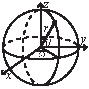
\includegraphics[width=25mm]{content/math/sphericalCoordinates}
\end{center}
\[\begin{array}{cc}
x = r\sin\theta\cos\phi & r = \sqrt{x^2+y^2+z^2}\\
y = r\sin\theta\sin\phi & \theta = \textrm{acos}(z/\sqrt{x^2+y^2+z^2})\\
z = r\cos\theta & \phi = \textrm{atan2}(y,x)
\end{array}\]

\subsection{Distances}
Manhattan $\to$ Chebyshev: $(x, y) \mapsto (x+y, x-y)$, then
$|x_1-x_2|+|y_1-y_2| = \max(|u_1-u_2|, |v_1-v_2|)$.

\section{Derivatives/Integrals}
\begin{align*}
	\dfrac{d}{dx}\arcsin x = \dfrac{1}{\sqrt{1-x^2}} &&& \dfrac{d}{dx}\arccos x = -\dfrac{1}{\sqrt{1-x^2}} \\
	\dfrac{d}{dx}\tan x = 1+\tan^2 x &&& \dfrac{d}{dx}\arctan x = \dfrac{1}{1+x^2} \\
	\int\tan ax = -\dfrac{\ln|\cos ax|}{a} &&& \int x\sin ax = \dfrac{\sin ax-ax \cos ax}{a^2} \\
	\int e^{-x^2} = \frac{\sqrt \pi}{2} \text{erf}(x) &&& \int xe^{ax}dx = \frac{e^{ax}}{a^2}(ax-1)
\end{align*}
Integration by parts:
\[\int_a^bf(x)g(x)dx = [F(x)g(x)]_a^b-\int_a^bF(x)g'(x)dx\]

\section{Sums}
\[ c^a + c^{a+1} + \dots + c^{b} = \frac{c^{b+1} - c^a}{c-1}, c \neq 1 \]
\begin{align*}
	1 + 2 + 3 + \dots + n &= \frac{n(n+1)}{2} \\
	1^2 + 2^2 + 3^2 + \dots + n^2 &= \frac{n(2n+1)(n+1)}{6} \\
	1^3 + 2^3 + 3^3 + \dots + n^3 &= \frac{n^2(n+1)^2}{4} \\
	1^4 + 2^4 + 3^4 + \dots + n^4 &= \frac{n(n+1)(2n+1)(3n^2 + 3n - 1)}{30} \\
	1 + \frac12 + \dots + \frac1n &\approx \ln n + 0.5772
\end{align*}

\section{Series}
$$e^x = 1+x+\frac{x^2}{2!}+\frac{x^3}{3!}+\dots,\,(-\infty<x<\infty)$$
$$\ln(1+x) = x-\frac{x^2}{2}+\frac{x^3}{3}-\frac{x^4}{4}+\dots,\,(-1<x\leq1)$$
$$\sqrt{1+x} = 1+\frac{x}{2}-\frac{x^2}{8}+\frac{2x^3}{32}-\frac{5x^4}{128}+\dots,\,(-1\leq x\leq1)$$
$$\sin x = x-\frac{x^3}{3!}+\frac{x^5}{5!}-\frac{x^7}{7!}+\dots,\,(-\infty<x<\infty)$$
$$\cos x = 1-\frac{x^2}{2!}+\frac{x^4}{4!}-\frac{x^6}{6!}+\dots,\,(-\infty<x<\infty)$$

\section{Probability theory}
Let $X$ be a discrete random variable with probability $p_X(x)$ of assuming the value $x$. It will then have an expected value (mean) $\mu=\mathbb{E}(X)=\sum_xxp_X(x)$ and variance $\sigma^2=V(X)=\mathbb{E}(X^2)-(\mathbb{E}(X))^2=\sum_x(x-\mathbb{E}(X))^2p_X(x)$ where $\sigma$ is the standard deviation. If $X$ is instead continuous it will have a probability density function $f_X(x)$ and the sums above will instead be integrals with $p_X(x)$ replaced by $f_X(x)$.

Expectation is linear, even for dependent variables:
\[\mathbb{E}(aX+bY) = a\mathbb{E}(X)+b\mathbb{E}(Y)\]
For independent $X$ and $Y$, \[V(aX+bY) = a^2V(X)+b^2V(Y).\]
\textbf{Tricks:} write a count as a sum of indicator variables and add their probabilities.
For integer $X\ge0$: $\mathbb{E}(X)=\sum_{k\ge1}P(X\ge k)$. Independent events: $P(A\cap B)=P(A)P(B)$;
$P(\text{at least one}) = 1 - P(\text{none})$. Bayes: $P(A|B)=P(B|A)P(A)/P(B)$.
Expected value DP: $E[s] = c(s) + \sum_t p(s\to t)E[t]$; with cycles, solve linear equations (Gauss.h).
Probabilities mod $p$: $a/b \to a\cdot b^{-1}$.

\subsection{Discrete distributions}

\subsubsection{Binomial distribution}
The number of successes in $n$ independent yes/no experiments, each which yields success with probability $p$ is $\textrm{Bin}(n,p),\,n=1,2,\dots,\, 0\leq p\leq1$.
\[p(k)=\binom{n}{k}p^k(1-p)^{n-k}\]
\[\mu = np,\,\sigma^2=np(1-p)\]
$\textrm{Bin}(n,p)$ is approximately $\textrm{Po}(np)$ for small $p$.

\subsubsection{First success distribution}
The number of trials needed to get the first success in independent yes/no experiments, each which yields success with probability $p$ is $\textrm{Fs}(p),\,0\leq p\leq1$.
\[p(k)=p(1-p)^{k-1},\,k=1,2,\dots\]
\[\mu = \frac1p,\,\sigma^2=\frac{1-p}{p^2}\]
Coupon collector ($n$ types): $n H_n \approx n\ln n$ draws.

\subsubsection{Poisson distribution}
The number of events occurring in a fixed period of time $t$ if these events occur with a known average rate $\kappa$ and independently of the time since the last event is $\textrm{Po}(\lambda),\,\lambda=t\kappa$.
\[p(k)=e^{-\lambda}\frac{\lambda^k}{k!}, k=0,1,2,\dots\]
\[\mu=\lambda,\,\sigma^2=\lambda\]

\subsection{Continuous distributions}

\subsubsection{Uniform distribution}
If the probability density function is constant between $a$ and $b$ and 0 elsewhere it is $\textrm{U}(a,b),\,a<b$.
\[f(x) = \left\{
\begin{array}{cl}
\frac{1}{b-a} & a<x<b\\
0 & \textrm{otherwise}
\end{array}\right.\]
\[\mu=\frac{a+b}{2},\,\sigma^2=\frac{(b-a)^2}{12}\]

\subsubsection{Exponential distribution}
The time between events in a Poisson process is $\textrm{Exp}(\lambda),\,\lambda>0$.
\[f(x) = \left\{
\begin{array}{cl}
\lambda e^{-\lambda x} & x\geq0\\
0 & x<0
\end{array}\right.\]
\[\mu=\frac{1}{\lambda},\,\sigma^2=\frac{1}{\lambda^2}\]

\subsubsection{Normal distribution}
Most real random values with mean $\mu$ and variance $\sigma^2$ are well described by $\mathcal{N}(\mu,\sigma^2),\,\sigma>0$.
\[ f(x) = \frac{1}{\sqrt{2\pi\sigma^2}}e^{-\frac{(x-\mu)^2}{2\sigma^2}} \]
If $X_1 \sim \mathcal{N}(\mu_1,\sigma_1^2)$ and $X_2 \sim \mathcal{N}(\mu_2,\sigma_2^2)$ then
\[ aX_1 + bX_2 + c \sim \mathcal{N}(\mu_1+\mu_2+c,a^2\sigma_1^2+b^2\sigma_2^2) \]

\section{Markov chains}
A \emph{Markov chain} is a discrete random process with the property that the next state depends only on the current state.
Let $X_1,X_2,\ldots$ be a sequence of random variables generated by the Markov process.
Then there is a transition matrix $\mathbf{P} = (p_{ij})$, with $p_{ij} = \Pr(X_n = i | X_{n-1} = j)$,
and $\mathbf{p}^{(n)} = \mathbf P^n \mathbf p^{(0)}$ is the probability distribution for $X_n$ (i.e., $p^{(n)}_i = \Pr(X_n = i)$),
where $\mathbf{p}^{(0)}$ is the initial distribution.

$\mathbf{\pi}$ is a stationary distribution if $\mathbf{\pi} = \mathbf{\pi P}$.
If the Markov chain is \emph{irreducible} (it is possible to get to any state from any state),
then $\pi_i = \frac{1}{\mathbb{E}(T_i)}$ where $\mathbb{E}(T_i)$  is the expected time between two visits in state $i$.
$\pi_j/\pi_i$ is the expected number of visits in state $j$ between two visits in state $i$.

For a connected, undirected and non-bipartite graph, where the transition probability is uniform among all neighbors, $\pi_i$ is proportional to node $i$'s degree.

A Markov chain is \emph{ergodic} if the asymptotic distribution is independent of the initial distribution.
A finite Markov chain is ergodic iff it is irreducible and \emph{aperiodic} (i.e., the gcd of cycle lengths is 1).
$\lim_{k\rightarrow\infty}\mathbf{P}^k = \mathbf{1}\pi$.

A Markov chain is an A-chain if the states can be partitioned into two sets $\mathbf{A}$ and $\mathbf{G}$, such that all states in $\mathbf{A}$ are absorbing ($p_{ii}=1$), and all states in $\mathbf{G}$ leads to an absorbing state in $\mathbf{A}$.
The probability for absorption in state $i\in\mathbf{A}$, when the initial state is $j$, is $a_{ij} = p_{ij}+\sum_{k\in\mathbf{G}} a_{ik}p_{kj}$.
The expected time until absorption, when the initial state is $i$, is $t_i = 1+\sum_{k\in\mathbf{G}}p_{ki}t_k$.

\section{Game theory}
\textbf{Nim:} the first player wins iff $a_1 \oplus \dots \oplus a_n \ne 0$.
\textbf{Sprague-Grundy:} $g(state) = \operatorname{mex}\{g(next)\}$; a sum of games
has $g = g_1 \oplus g_2 \oplus \dots$; losing iff $g = 0$.
Staircase nim: only odd steps matter. Misere nim: like nim, unless all piles are
$\le 1$ (then the first player wins iff the number of piles is even).
Taking $1..k$ stones from one pile: $g(n) = n \bmod (k+1)$.
Symmetric boards: the second player can often mirror the first.
